\documentclass[tikz,border=10pt]{standalone}
\usepackage{tikz}
\usetikzlibrary{arrows.meta,positioning,calc,patterns}

\begin{document}
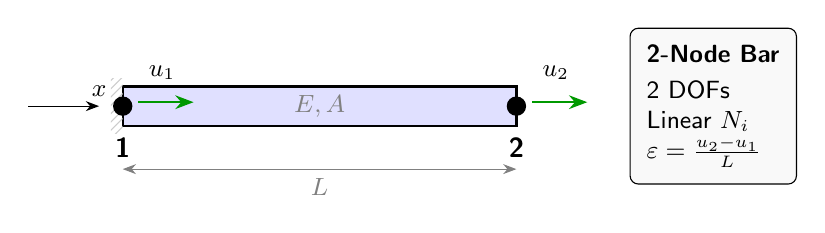
\begin{tikzpicture}[
    node font=\sffamily,
    >=Stealth,
    node dot/.style={circle, fill=black, inner sep=0pt, minimum size=7pt},
    dof arrow/.style={->, thick, color=green!60!black},
]

% Bar element body
\fill[blue!12] (0,-0.25) rectangle (5,0.25);
\draw[thick] (0,-0.25) rectangle (5,0.25);

% Cross-hatching for cross-section indication
\fill[pattern=north east lines, pattern color=gray!40] (-0.15,-0.35) rectangle (0,0.35);

% Nodes
\node[node dot] (n1) at (0,0) {};
\node[node dot] (n2) at (5,0) {};

% Node labels
\node[below=8pt, font=\bfseries] at (n1) {1};
\node[below=8pt, font=\bfseries] at (n2) {2};

% DOF arrows
\draw[dof arrow] (0.2,0.05) -- ++(0.7,0);
\draw[dof arrow] (5.2,0.05) -- ++(0.7,0);

% DOF labels
\node[above=6pt, font=\small\itshape] at (0.5,0) {$u_1$};
\node[above=6pt, font=\small\itshape] at (5.5,0) {$u_2$};

% Length dimension
\draw[<->, thin, gray] (0,-0.8) -- (5,-0.8) node[midway, below, font=\small\itshape] {$L$};

% Property labels
\node[font=\small\itshape, gray] at (2.5,0) {$E, A$};

% Coordinate axis
\draw[->] (-1.2,0) -- (-0.3,0) node[above, font=\small\itshape] {$x$};

% Info box
\node[draw, rounded corners=3pt, fill=gray!5, inner sep=6pt, font=\small, align=left] 
    at (7.5,0) {
    \textbf{2-Node Bar}\\[2pt]
    2 DOFs\\
    Linear $N_i$\\
    $\varepsilon = \frac{u_2 - u_1}{L}$
};

\end{tikzpicture}
\end{document}
